\documentclass[a0paper,portrait]{baposter}

% Packages nécessaires
\usepackage[utf8]{inputenc}
\usepackage[T1]{fontenc}
\usepackage[french]{babel}
\usepackage{graphicx}
\usepackage{xcolor}
\usepackage{tikz}
\usepackage{multicol}
\usepackage{adjustbox}
\usepackage{qrcode}
% \usepackage{fontawesome5} % Removed due to compatibility issues
\usepackage{lmodern}

% Configuration des couleurs
\definecolor{c4dtblue}{RGB}{0,102,179}
\definecolor{gnugengray}{RGB}{85,85,85}
\definecolor{lightblue}{RGB}{173,216,230}
\definecolor{darkgray}{RGB}{64,64,64}
\definecolor{lightgray}{RGB}{240,240,240}

% Configuration du poster
\begin{document}
\begin{poster}{
  % Options du poster
  columns=2,
  colspacing=1em,
  bgColorOne=white,
  bgColorTwo=white,
  borderColor=c4dtblue,
  headerColorOne=c4dtblue,
  headerColorTwo=lightblue,
  headerFontColor=white,
  boxColorOne=white,
  boxColorTwo=lightgray,
  textborder=rounded,
  eyecatcher=true,
  headerheight=0.08\textheight,
  headershape=rounded,
  headerfont=\Large\bf\textsf,
  textfont={\setlength{\parindent}{0em}\large},
  boxshade=plain,
  background=plain,
  linewidth=2pt
}
% Logo en haut à gauche
{
\includegraphics[height=6em]{assets/logos/C4DT_logo.png}}
% Titre principal
{\bf\textsf{\color{white}\huge Reprenez le contrôle de votre vie numérique}}
% Auteurs
{\textsf{\color{white}\huge Découvrez des alternatives respectueuses de votre vie privée}\\
\vspace{0.5em}
\textsf{\color{white}\Large Centre pour la Confiance Numérique (C4DT) - gnugen - digiges}}
% Logos en haut à droite
{\raisebox{-1em}{
\includegraphics[height=4em]{assets/logos/gnugen_logo.png}}\quad\raisebox{-1em}{
\includegraphics[height=4em]{assets/logos/digiges_logo.png}}}

% Contenu principal du poster
\headerbox{Êtes-vous client ou produit ?}{name=intro,column=0,row=0}{
  \vspace{0.5em}
  \begin{center}
  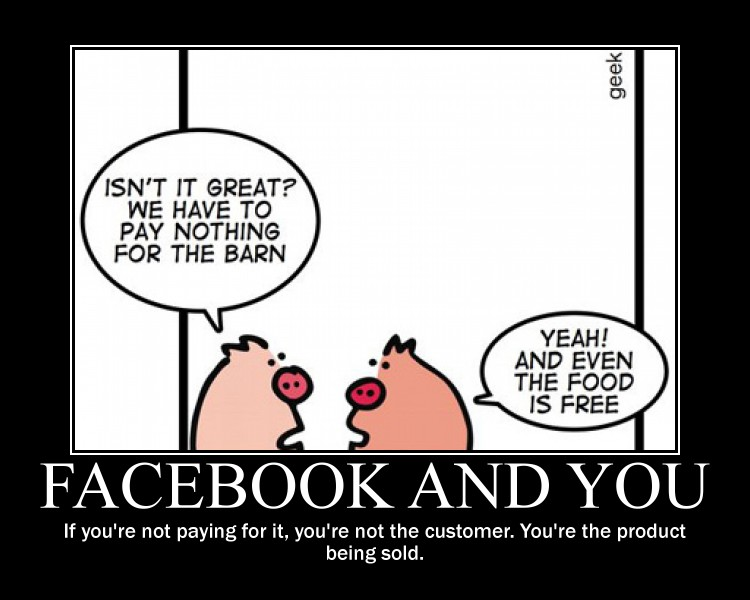
\includegraphics[width=0.8\textwidth]{assets/youre-the-product.jpg}
  \end{center}
  
  \textbf{\huge Votre vie privée : un droit fondamental}
  
  \textit{\Large Constitution Fédérale Suisse, Article 13 :}
  
  \textcolor{darkgray}{\large "Toute personne a droit au respect de sa vie privée et familiale, de son domicile, de sa correspondance et des relations qu'elle établit par la poste et les télécommunications."}
  
  \vspace{1em}
  
  \textbf{\color{c4dtblue}\LARGE Reprenez le contrôle !}
  \begin{itemize}
  \item{ Des alternatives libres existent}
  \item{ Protégez-vous sans sacrifier la simplicité}
  \item{ Vos données valent de l'or}
  \end{itemize}
}

\headerbox{Prenez conscience des enjeux}{name=stats,column=0,below=intro}{
  \textbf{\color{red}\Large E-mail :}
  \begin{itemize}
  \item{ 251 millions d'emails/minute}
  \item{ \textbf{3,4 milliards} d'emails de phishing quotidiens}
  \end{itemize}
  
  \textbf{\color{red}\Large Surveillance :}
  \begin{itemize}
  \item{ Profilage comportemental}
  \item{ Données vendues aux gouvernements}
  \item{ Ciblage publicitaire invasif}
  \end{itemize}
  
  \textbf{\color{red}\Large Monopolisation :}
  \begin{itemize}
  \item{ Concentration du pouvoir}
  \item{ Contrôle de l'information}
  \item{ Restriction des libertés numériques}
  \end{itemize}
}

\headerbox{Communications en Ligne}{name=communication,column=1,row=0}{
  \noindent
  \begin{minipage}[b]{0.7\linewidth}
    \textbf{\color{c4dtblue}X $\rightarrow$ Mastodon}
    \begin{itemize}
      \item Choisissez vos propres intérêts
      \item Pas de publicités
    \end{itemize}
  \end{minipage}%
  \begin{minipage}[t]{0.28\linewidth}
    \hspace{0.5em}
    \qrcode[height=2cm]{https://mastodon.social}
  \end{minipage}

  \vspace{0.5em}

  \noindent
  \begin{minipage}[t]{0.28\linewidth}
    \qrcode[height=2cm]{URL_HERE}
  \end{minipage}%
  \begin{minipage}[t]{0.7\linewidth}
    \hspace{0.5em}
    \textbf{\color{c4dtblue}WhatsApp $\rightarrow$ Signal}
    \begin{itemize}
      \item 
    \end{itemize}
  \end{minipage}

  \vspace{0.5em}

  \noindent
  \begin{minipage}[t]{0.7\linewidth}
    \textbf{\color{c4dtblue}Slack $\rightarrow$ Matrix}
    \begin{itemize}
      \item 
    \end{itemize}
  \end{minipage}%
  \begin{minipage}[t]{0.28\linewidth}
    \hspace{0.5em}
    \qrcode[height=2cm]{URL_HERE}
  \end{minipage}
}

\headerbox{Bureautique}{name=office,column=1,below=communication}{
  \noindent
  \begin{minipage}[t]{0.7\linewidth}
    \textbf{\color{c4dtblue}MS365 $\rightarrow$ K-Drive}
    \begin{itemize}
      \item Données stockées en Suisse (lois strictes)
      \item Pas d'analyse de vos fichiers pour la publicité
      \item Chiffrement de bout-en-bout disponible
    \end{itemize}
  \end{minipage}%
  \begin{minipage}[t]{0.28\linewidth}
    \hspace{0.5em}
    \qrcode[height=2cm]{URL_HERE}
  \end{minipage}

  \vspace{0.5em}

  \noindent
  \begin{minipage}[t]{0.28\linewidth}
    \qrcode[height=2cm]{URL_HERE}
  \end{minipage}%
  \begin{minipage}[t]{0.7\linewidth}
    \hspace{0.5em}
    \textbf{\color{c4dtblue}Outlook $\rightarrow$ Thunderbird}
    \begin{itemize}
      \item Aucune collecte de métadonnées
      \item Open source = transparence totale
      \item Fonctionne avec tous les fournisseurs email
    \end{itemize}
  \end{minipage}

  \vspace{0.5em}

  \noindent
  \begin{minipage}[t]{0.7\linewidth}
    \textbf{\color{c4dtblue}Chrome $\rightarrow$ Firefox}
    \begin{itemize}
      \item Bloque le tracking par défaut
      \item Moteur indépendant (pas Google)
      \item Extensions anti-pub plus efficaces
    \end{itemize}
  \end{minipage}%
  \begin{minipage}[t]{0.28\linewidth}
    \hspace{0.5em}
    \qrcode[height=2cm]{URL_HERE}
  \end{minipage}
}

\headerbox{Sécurité}{name=security,column=1,below=office}{
  \noindent
  \begin{minipage}[t]{0.7\linewidth}
    \textbf{\color{c4dtblue}Gestion de mots de passe}
    \begin{itemize}
      \item 
    \end{itemize}
  \end{minipage}%
  \begin{minipage}[t]{0.28\linewidth}
    \hspace{0.5em}
    \qrcode[height=2cm]{URL_HERE}
  \end{minipage}

  \vspace{0.5em}

  \noindent
  \begin{minipage}[t]{0.28\linewidth}
    \qrcode[height=2cm]{URL_HERE}
  \end{minipage}%
  \begin{minipage}[t]{0.7\linewidth}
    \hspace{0.5em}
    \textbf{\color{c4dtblue}Non aux pubs avec uBlock}
    \begin{itemize}
      \item 
    \end{itemize}
  \end{minipage}

  \vspace{0.5em}

  \noindent
  \begin{minipage}[t]{0.7\linewidth}
    \textbf{\color{c4dtblue}Consent-o-matic}
    \begin{itemize}
      \item 
    \end{itemize}
  \end{minipage}%
  \begin{minipage}[t]{0.28\linewidth}
    \hspace{0.5em}
    \qrcode[height=2cm]{URL_HERE}
  \end{minipage}
}

% \headerbox{Gestionnaires de mots de passe}{name=passwords,column=0,below=intro}{
%   \textbf{\Large Essentiel en 2025 !}
  
%   \vspace{0.5em}
  
%   \textbf{\color{c4dtblue}Synchronisation multi-appareils :}
%   \begin{itemize}
%   \item \textbf{Bitwarden/Vaultwarden} - Gratuit, open source
%   \item Plan gratuit avec mots de passe illimités
%   \item Export de données possible
%   \end{itemize}
  
%   \textbf{\color{c4dtblue}Usage local uniquement :}
%   \begin{itemize}
%   \item \textbf{KeePassXC} - Multi-plateforme, gratuit
%   \item Android : KeePassDX
%   \item iOS : KeePassium ou AuthPass
%   \end{itemize}
  
%   \textbf{\color{c4dtblue}Authentification à deux facteurs (2FA) :}
%   \begin{itemize}
%   \item Aegis (Android)
%   \item OpenOTP (Android \& iOS)
%   \item GNOME Authenticator (Linux)
%   \end{itemize}
  
%   \textbf{IMPORTANT :}
%   \begin{itemize}
%   \item Faites des sauvegardes régulières
%   \item Mot de passe maître fort
%   \item Évitez les SMS pour la 2FA
%   \end{itemize}
% }

% \headerbox{Navigateurs et Extensions}{name=browsers,column=1,row=0}{
%   \textbf{\Large Protégez-vous en naviguant}
  
%   \vspace{0.5em}
  
%   \textbf{\color{c4dtblue}Navigateurs recommandés :}
%   \begin{itemize}
%   \item \textbf{Firefox} - Indépendant, open source
%   \item Moteur Gecko (pas Chrome/Blink)
%   \item Anti-Manifest V3
%   \item \textbf{LibreWolf} - Firefox durci
%   \item Protection renforcée
%   \item Cookies supprimés automatiquement
%   \end{itemize}
  
%   \textbf{\color{c4dtblue}Extensions essentielles :}
%   \begin{itemize}
%   \item \textbf{uBlock Origin} - Bloque publicités et trackers
%   \item Protection contre liens malveillants
%   \item \textbf{Consent-O-Matic} - Refuse automatiquement les cookies
%   \item \textbf{Cookie AutoDelete} - Garde seulement les cookies nécessaires
%   \end{itemize}
  
%   \vspace{1em}
  
%   \textbf{LE SAVIEZ-VOUS ?}
  
%   \textcolor{darkgray}{Chrome/Blink contrôle 70\% du web. Le passage à Manifest V3 limite le blocage des publicités et trackers. Firefox reste indépendant !}
% }

% \headerbox{Messagerie \& Réseaux Sociaux}{name=social,column=1,below=browsers}{
%   \textbf{\color{c4dtblue}Messagerie chiffrée :}
%   \begin{itemize}
%   \item \textbf{Matrix} (matrix.epfl.ch) - Fédéré, chiffrement bout-à-bout
%   \item \textbf{Signal} - Mobile, très sécurisé
%   \item Alternative à WhatsApp/Telegram
%   \end{itemize}
  
%   \textbf{\color{c4dtblue}Réseaux sociaux fédérés :}
%   \begin{itemize}
%   \item \textbf{Mastodon} (social.epfl.ch) - Alternative à Twitter/X
%   \item Pas d'algorithme manipulateur
%   \item Contrôle de votre fil d'actualité
%   \end{itemize}
  
%   \textbf{\color{c4dtblue}Visioconférence :}
%   \begin{itemize}
%   \item \textbf{Jitsi} - Alternative à Zoom
%   \item \textbf{Element Call} - Intégré à Matrix
%   \end{itemize}
% }

% \headerbox{Stockage \& Bureautique}{name=office,column=2,row=0}{
%   \textbf{\color{c4dtblue}Stockage en ligne :}
%   \begin{itemize}
%   \item \textbf{Infomaniak kDrive} - Suisse, respectueux
%   \item Alternative à Google Drive/OneDrive
%   \item \textbf{Nextcloud} - Auto-hébergeable
%   \item Contrôle total de vos données
%   \end{itemize}
  
%   \textbf{\color{c4dtblue}Suite bureautique :}
%   \begin{itemize}
%   \item \textbf{LibreOffice} - Riche en fonctionnalités
%   \item \textbf{OnlyOffice} - Interface similaire à MS Office
%   \item Meilleure compatibilité
%   \end{itemize}
  
%   \textbf{\color{c4dtblue}Client email :}
%   \begin{itemize}
%   \item \textbf{Thunderbird} - Alternative libre à Outlook
%   \item Multi-comptes, extensions
%   \end{itemize}
  
%   \textbf{\color{c4dtblue}Intelligence Artificielle :}
%   \begin{itemize}
%   \item \textbf{En ligne :} Duck.ai, Lumo (Proton)
%   \item \textbf{Local :} LM Studio, Ollama
%   \item Gardez vos données privées
%   \end{itemize}
% }

\headerbox{Venez discuter avec nous !}{name=contact,column=0,span=2,above=bottom}{
  \begin{multicols}{3}
  \textbf{\Large Nous sommes là pour vous aider}
  
  \textbf{\color{c4dtblue}Qui sommes-nous ?}
  \begin{itemize}
  \item \textbf{C4DT} - Centre pour la Confiance Numérique
  \item \textbf{gnugen} - Promotion du logiciel libre à l'EPFL
  \item \textbf{digiges} - Partenaire pour la transition numérique
  \end{itemize}
  
  \columnbreak
  
  \textbf{\color{c4dtblue}Questions fréquentes :}
  \begin{itemize}
  \item Comment choisir un gestionnaire de mots de passe ?
  \item Firefox ou LibreWolf pour débuter ?
  \item Comment migrer depuis Google/Microsoft ?
  \item Quel niveau de sécurité me convient ?
  \end{itemize}
  
  \columnbreak
  
  \textbf{\color{c4dtblue}Ressources utiles :}
  
  \begin{center}
  \qrcode[height=3cm]{https://gnugen.ch/fr/guides/}
  
  \textbf{Guide de survie numérique}
  
  \texttt{gnugen.ch/fr/guides/}
  
  \vspace{1em}
  
  \textbf{Contact :} 
  Carine Dengler \\
  Linus Gasser\\
  Centre pour la Confiance Numérique
  \end{center}
  
  \end{multicols}
}

\end{poster}
\end{document}
